\documentclass{beamer}
\usepackage[latin1]{inputenc}
\usepackage{amsfonts}
%\usetheme{Luebeck}
\usetheme{Warsaw}
\title[Patient Service System]{Patient Service System}
%\subtitle{CS308 Project Presentation I}

\author {CS308 Project Presentation I}
\date{Group Members :}
\begin{document}
\begin{frame}
\titlepage
\begin{center}
\medskip
\begin{tabular}{lllll}
Pritish Kamath & (08005004) & & Rohit Saraf &  (08005040) \\
Ashish Mathew  &  (08d10035) & & Vivek Madan &  (08005035)\\\
\end{tabular}\\
under the guidance of\\
\begin{large}
\textbf{Prof. Kavi Arya}
\end{large}
\end{center}
\end{frame}

%\author {CS308 Project Presentation I}
%\date{by}
%\begin{document}
%\begin{frame}
%\titlepage
%\begin{center}
%%\begin{large}
%\medskip
%\begin{tabular}{ll}
%Pritish Kamath & 08005004 \\
%Rohit Saraf &  08005040 \\
%Vivek Madan  &  08005035\\
%Ashish Mathew &  08d10035\\\
%\end{tabular}
%%\end{large} \\
%under the guidance of\\
%\begin{large}
%\textbf{Prof. Kavi Arya}\\
%\end{large}
%\end{center}
%\end{frame}

\section{Problem Statement and Description}
\subsection{Problem Statement}
\begin{frame}{Patient Service System - Problem Statement}
\begin{enumerate}
\item Automatic attendants which would serve patients' requests such as supplying water or patient specific medicines etc.
\item These attendants should be summonable using an easy to use interface by the patients.
\item The patients should be served in a fair-share manner and the requests should satisfy bounded wait.
\end{enumerate}
\end{frame}

\subsection{Description}
\begin{frame}{Patient Service System - Description}
\begin{enumerate}
\item Each patient has a TV remote with which he/she can send a request to the server.
\item On receiving a request, the server sends a bot to serve the patients' requests. This is communicated to the patient via an SMS.
\item The server ensures reliable communication (via Zigbee) with all the serving bots and the patient controller.
\item The server design must be scalable to serve a large number of patients, and must be free of deadlocks, race conditions and must have maximum concurrency.
\item If a bot is blocked on it's path to the patient, then the server informs the security about the block, via an SMS.
\end{enumerate}
\end{frame}

\section{Functional Requirements and Execution}
\subsection{Functional Requirements}
\begin{frame}{Functional Requirements}
\begin{enumerate}
\item Central Server
\begin{itemize}
\item Patient requests should be communicated to the centralized server through a wireless medium.
\item  The centralized server would send attendants to serve the patients' requests or communicate to doctors about the urgency of the situation (through SMS or otherwise), whichever applicable.
\item  It should run a scheduling algorithm to manage the robotic attendants so as to serve the patients in a least possible time.
\end{itemize}
\item Robotic Attendants
\begin{itemize}
\item  The robot should follow a fixed path indicated by white lines.
\item  It should stop in presence of an obstruction and alarm the guards about its prolonged obstructed movement and send an SMS (through the server) to inform the security.
\item  It should be able to serve multiple patients, on request.
\end{itemize}
\end{enumerate}
\end{frame}   

\subsection{Work Execution}
\begin{frame}{Work Execution (1/2)}
\begin{itemize}
\item Got Zigbee communication working with Java. (2 days)
\item Making Arena and perfecting White Line Follower (7-fold algorithm with error recovery) (2 days)
\item Designing Polling based communication protocol : both server and bot. (1 day)
\item Creating MySQL Database for patient requests, and designing Bot Locomotion algorithm (ensuring no deadlocks and bot-bot collisions). (2 days)
\item Simulation (with rigorous testing - independent of the bot) of the server. Checking for deadlocks and race conditions. (2 days)
\end{itemize}
\end{frame}

\begin{frame}{Work Execution (2/2)}
\begin{itemize}
\item Taking input from \emph{TV remote} for patient requests. Designing a \emph{Protocol independent Learning based Algorithm} for capturing inputs. (2 days)
\item Sending \emph{SMS} through python script. (1 day)
\item Writing scripts for configuring the system for setting up all necessary softwares. (1 day)
\item Documenting all code (using Doxygen tool), writing readme file and making the final presentation (1 day).
\end{itemize}
\end{frame}

\subsection{Work Division}
\begin{frame}{Work Division (1/2)}
\begin{tabular}{|l|l|}
\hline
\textbf{Work/Critical Tasks} & \textbf{People responsible} \\
\hline
\hline
Zigbee communication with Java & Vivek Madan,\\ & Rohit Saraf,\\ & Ashish Mathew \\
\hline
Making Arena & Pritish Kamath, \\
Perfecting Line Follower & Rohit Saraf \\
\hline
Implementing Server Side Polling based & Vivek Madan, \\
Communication Protocol & Ashish Mathew \\
\hline
Implementing Bot Side Polling based & Pritish Kamath, \\
Communication Protocol & Rohit Saraf \\
\hline
\end{tabular}
\end{frame}

\begin{frame}{Work Division (2/2)}
\begin{tabular}{|l|l|}
\hline
\textbf{Work/Critical Tasks} & \textbf{People responsible} \\
\hline
\hline
MySQL Database for patients & Vivek Madan, \\
Bot Locomotion Algorithm (server) & Ashish Mathew \\
Simulation & \\
\hline
Taking input from TV remote & Pritish Kamath,\\
Sending SMS via Python Script (internet) & Rohit Saraf,\\
\hline
Configure Scripts and Makefile & Rohit Saraf \\
\hline
Documentation & All \\
\hline
\end{tabular}
\begin{itemize}
\item[]
\end{itemize}
Project Completion Date : 5th April 2011
\end{frame}

\section{Finite State Machine}
\begin{frame}{Bot FSM}
\begin{figure}
\centerline{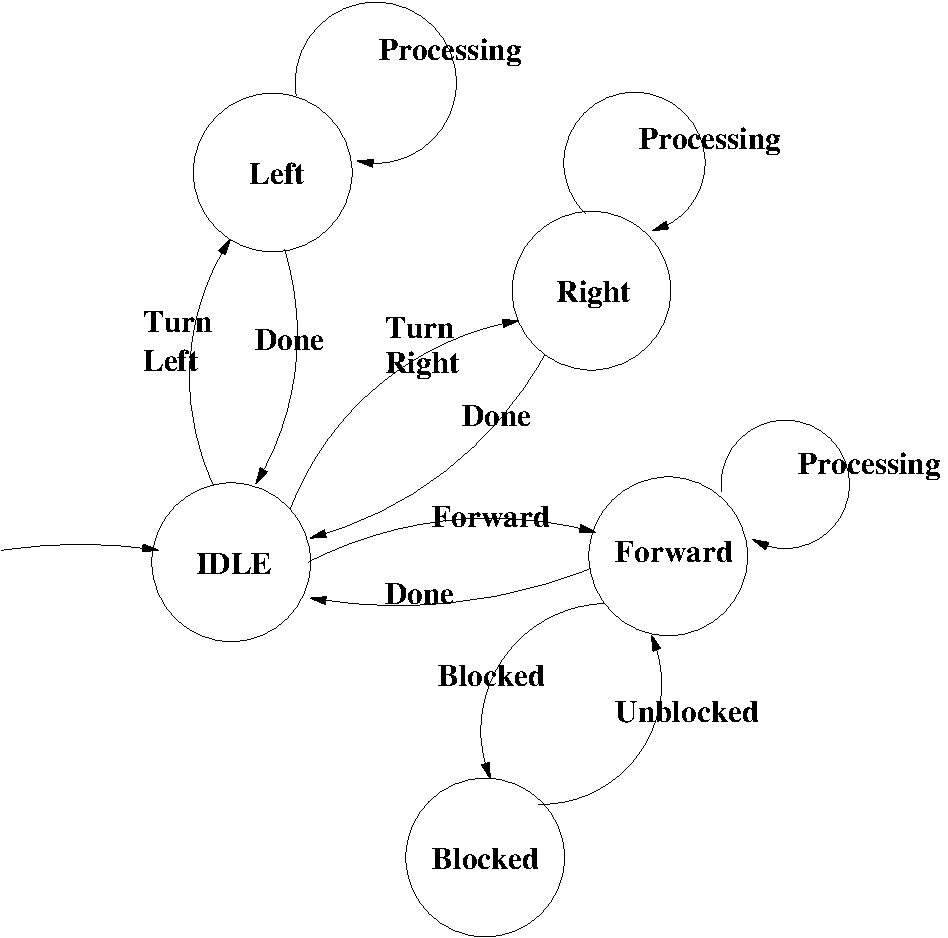
\includegraphics[scale=0.35]{fsm.pdf}}
\caption{Service Bot FSM}\label{fig:exp}
\end{figure}
\end{frame}

\section{Innovations, Challenges and Solutions}
\subsection{Innovations and Challenges}
\begin{frame}{Innovation and Challenges (1/2)}
\begin{itemize}
\item Server runs in Ubuntu. Bot AVR-programming done in Ubuntu.
\item Zigbee communication using \emph{Java}.
\item MySQL database. Makes the project scalable for large number of patients.
\item Correction and Recovery while following the white line. Smooth running of the bot, (without any extra squares added at intersections).
\item Polling based communication implemented to avoid interference between serving bot and patient bot.
\end{itemize}
\end{frame}

\begin{frame}{Innovation and Challenges (2/2)}
\begin{itemize}
\item Maximum parallelism and concurrency to avoid time/resource wastage. (Multithreading which is not concurrent like pthread, but actually parallel).
\item Testing everything and making the design modular so that the different parts have least to do with one another. Done using virtual simulation of bots.
\item Ensuring no deadlock between multiple bots.
\item Getting TV remote to work using a Protocol independent learning based algorithm.
\item Sending SMS to phone.
\item Efficient Scheduling Algorithm.
\end{itemize}
\end{frame} 

\subsection{Problems and Solutions}
\begin{frame}{Problems Faced and Solutions (1/2)}
\begin{tabular}{|l|l|}
\hline
\textbf{Problems faced} & \textbf{Devised Solutions} \\
\hline
\hline
Line following not working reliably & 7-fold algorithm employing \\
& Error Correction and Recovery \\
\hline
Simultaneous Zigbee communication & Polling based protocol \\
with two other Zigbee modules & \\
\hline
Delay required after sending data & Multithreaded server : \\
via Zigbee causes problem in & Separate thread for \\
execution of Graph algorithm & each send operation \\
\hline
\end{tabular}
\end{frame}

\begin{frame}{Problems Faced and Solutions (2/2)}
\begin{tabular}{|l|l|}
\hline
\textbf{Problems faced} & \textbf{Devised Solutions} \\
\hline
\hline
TV remote protocol not reliable & Use Protocol independent \\
& Learning based algorithm \\
\hline
IR-interrupt conflicting with & Do IR checking in a busy \\
USART sensor & wait manner.\\
\hline
A large files causing problems & Configure Scripts and Makefile \\
in compilation and setup & \\
\hline
\end{tabular}
\begin{itemize}
\item[]
\end{itemize}
\end{frame}

\section{Testing Strategy}
\subsection{Arena}
\begin{frame}{Arena}
\begin{figure}
\centerline{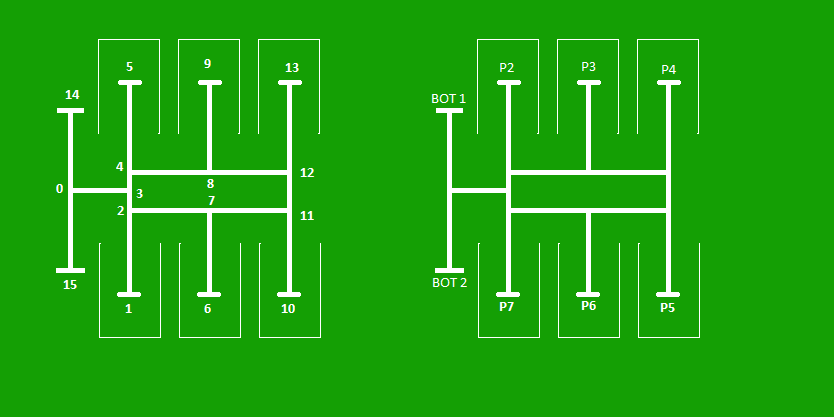
\includegraphics[scale=0.45]{Arena.png}}
\caption{Arena}\label{fig:exp}
\end{figure}
\end{frame}

\subsection{Modular Testing}
\begin{frame}{Modular Testing}
\begin{itemize}
\item Testing multiple Zigbee client - single Zigbee server protocol.
\item Virtual bot simulation and testing of server.
\item Testing for deadlocks and race conditions.
\item Server independent testing of serving bots.
\item Independent TV remote testing.
\end{itemize}
\end{frame}

\subsection{Combined Testing}
\begin{frame}{Combined Testing}
\begin{itemize} 
\item Correct patient-request is served by the attendant.
\item Attendant stops in presence of obstruction and beeps in case of prolonged obstruction.
\item 6 patient controllers using TV remote.
\item Simultaneous requests allowed (served in fair-share FIFO order).
\end{itemize}
\end{frame}

\section{Code Reusability}
\begin{frame}{Code Reusability}
\begin{enumerate} 
\item Server code : Completely object oriented (Java).
\item Modular Design : Modules independent of each other, hence can be changed without changing others.
\begin{itemize}
\item A different arena can be stored by changing \emph{Graph.java}.
\item Polling protocol can be changed by changing \emph{PollingThread.java}.
\item \emph{Properties} file stores all user dependent constants that can be changed without going through/compiling the code.
\end{itemize}
\item Server is bot-hardware independent. Relies on only a serial communication protocol (not necessarily Zigbee) with the bot.
\end{enumerate}
\end{frame}

\begin{frame}{Future Directions}
\begin{itemize} 
\item Can be adapted to suit hospitals like Tata Memorial Hospital.
\item Attendants can be suited to check patient condition (such as glucose bottle levels) and take appropriate action (refill the glucose bottle).
\item Can be used to help in house-hold activities (such as watering plants, etc.). TV remote based interface makes it convenient to use.
\end{itemize}
\end{frame}

\end{document}
